\documentclass[a4paper,11pt]{scrartcl}

\usepackage[utf8]{inputenc} %-- pour utiliser des accents en français
\usepackage{graphicx} % les graphiques
\usepackage{mathpazo} % la police
\usepackage{float} % pour avoir l'option H sur les figures
\usepackage{listings}  % partie de code

% Pour les tableaux 
\usepackage{array,multirow,makecell}
\makegapedcells
\usepackage[table]{xcolor}
\setcellgapes{1pt}
\newcolumntype{R}[1]{>{\raggedleft\arraybackslash }b{#1}}
\newcolumntype{L}[1]{>{\raggedright\arraybackslash }b{#1}}
\newcolumntype{C}[1]{>{\centering\arraybackslash }b{#1}}


% Packages nécessaires pour la bibliographie
\usepackage{hyperref}  % Pour les hyperliens
\usepackage{url}       % Pour la gestion des URLs

% ///////////////////////////////////////////////////

\begin{document}
\title{
    Aide d'utilisation du plugin "OSI Projets"\\
    Version 1.1.28
}

\author{}
\date{}
\maketitle


\begin{tabular}{|>{\centering\arraybackslash    \columncolor{lightgray} 
    }m{4cm}|>{\centering\arraybackslash}m{10cm}|}
    \hline
    version & 1.1.28 \\ 
    \hline
    etat & dev \\ 
    \hline
    GitHub du plugin &\href{https://github.com/TuilierGit/osi_projets}{https://github.com/TuilierGit/osi\_projets} \\ 
    \hline
    Documents sur plugin &\href{https://github.com/TuilierGit/osi_projets_documents}{https://github.com/TuilierGit/osi\_projets\_documents}\\ 
    \hline
\end{tabular}\\

\newpage


\section{Introduction} \label{section:introduction}
Nous allons ici présenter le plugin Spip nommé \textbf{OSI Projets}. Ce plugin a pour objectif de pouvoir mettre en place un système de gestion de projets au sein d'un site Spip. La version présentée ici est la version \texttt{1.1.28} qui est encore une version de développement. C'est à-dire que le projet peut encore posséder certains bugs qu'il ne faut pas hésiter à déclarer, voire à directement corriger via le GitHub. À savoir que le plugin est accessible sur la page GitHub suivante :
\begin{center}
    \href{https://github.com/TuilierGit/osi_projets}{https://github.com/TuilierGit/osi\_projets}
\end{center}


\subsection{Histoire du plugin}

Ce plugin a été réalisé à la demande de l'ONG "OBJECTIF SCIENCES International" (OSI). Il a été réalisé dans sa première version durant un stage en 2024 par Thomas Tuilier.

\subsection{Objectifs du plugin}
Les objectifs de ce plugin sont les suivants : 
\begin{itemize}
    \item Les projets doivent pouvoir regrouper différents participants, chacun ayant plus ou moins de droits sur les projets.
    \item Chaque projet doit pouvoir ajouter des critères d’entrée et définir un certain agencement entre eux, c’est-à-dire un ordre de participation aux projets.
    \item Les projets peuvent être considérés comme des formations, ils doivent donc permettre de définir des récompenses pout les participants. 
    \item Il doit être possible d'ajouter des rôles aux membres d'un projet.
    \item Un projet doit pouvoir être visible sur le front du site.
\end{itemize}



\newpage

\section{Installation du plugin} \label{section:introduction}
Ce plugin s'installe de la même manière que les autres plugins SPIP, c’est-à-dire dans le dossier \texttt{www/plugins} du site SPIP ou directement via l'installation du back-office.\\
\newline
Une fois le plugin installé, il est important de sélectionner la configuration adaptée au site dans le menu de configuration du plugin (Cf partie \ref{section:back-office}).

% \newpage

\section{Règles du plugin} \label{section:regles}
Pour utiliser le plugin, il faut connaître certaines règles qui ont été définies avec celui-ci :
\begin{itemize}
    \item Le créateur du projet ne peut pas quitter le projet. Il est considéré comme un super-administrateur, c'est la seule personne qui peut exclure n'importe quel membre du projet, administrateur ou non. Il peut modifier l'état de n'importe quel membre du projet.
    \item Les administrateurs peuvent exclure, ajouter des utilisateurs (accepter la demande), ou modifier les droits des autres utilisateurs sur ce projet. Ils peuvent aussi modifier les critères d'entrée et de récompenses du projet.
\end{itemize}

\newpage

\section{Gestion front} \label{section:front-office}
Il existe différentes manières d'intéragir avec le plugin sur le front. Le plus simple est d'utiliser la structure déjà proposée avec le plugin. Pour faire cela, il suffit de rajouter dans le squelette des rubriques (le fichier \texttt{rubrique.html} du dossier \texttt{squelettes} du site) la ligne suivante : 
\begin{lstlisting}
    <INCLURE{fond=inclure/page-projets,id_rubrique=#ID_RUBRIQUE 
    ,env,ajax,cache=0}/>
\end{lstlisting}
À cet emplacement apparaîtra :
\begin{itemize}
    \item Le bouton de création de projet, si c'est une rubrique définie dans la configuration du plugin.
    \item Le menu du projet, si c'est une rubrique associée à un projet.
    \item La liste des sous-projets.
\end{itemize}

\newpage

\section{Gestion back-office} \label{section:back-office}
Lors de l'installation du plugin, deux menus s'ajoutent sur la partie \textit{back-office}. Le premier se trouve dans le menu \textbf{Édition} et le deuxième dans le menu \textbf{Configuration}. 

\subsection{Menu configuration} \label{subsection:configuration}

Dans le menu configuration se trouvent trois sous-menus :
\begin{itemize}
    \item Diverses options
    \item Gestion des rôles
    \item Gestion des notifications
\end{itemize}
Nous allons revenir sur ces différents menus.

\subsubsection*{Diverses options} \label{subsubsection:diverses-options}
Dans ces sous-menus, il est possible de définir différents paramètres. Ces paramètres sont censés offrir des possibilités d'adaptation du plugin aux besoins du site. Nous allons les expliquer un par un. Pour chaque configuration, le système de configuration SPIP a été utilisé. Les configurations sont donc accessible dans le code via les fonctions \texttt{ecrire\_config} et \texttt{lire\_config}.\\
\newline
Le fichier \texttt{action/exemple\_configuration.php} offre une configuration d'exemple déjà définie. Il est possible de l'utiliser en passant par le bouton du menu nommé "\textit{Utiliser la configuration d'exemple}". Cependant il est toujours préférable de réaliser une configuration adaptée au site.\\
\newline
Pour chaque configuration, la valeur prend soit 0, soit 1. Si la valeur est à 0 (valeur initiale) alors l'option n'est pas activée, sinon, si l'option est sur 1, alors elle est activée.

\newpage
% ///////////////////////////////////


\textbf{Option 1 :} 
\begin{itemize}
    \item Configuration : \texttt{osi\_projets/rubriques/N} avec N l'indice de la rubrique
    \item Explication : Cette option comporte deux groupes de rubrique, le premier groupe représente les rubriques classiques et le deuxième groupe représente toutes les rubriques dans lesquelles il est possible de créer un projet sur le front (sans parler de sous projet, Cf option \ref{option9}. Il n'est pas nécessaires qu'une rubrique soit une rubrique de création pour voir ses sous projets)
\end{itemize}
\vspace{0.5cm}
\begin{figure}[h]
    \centering
    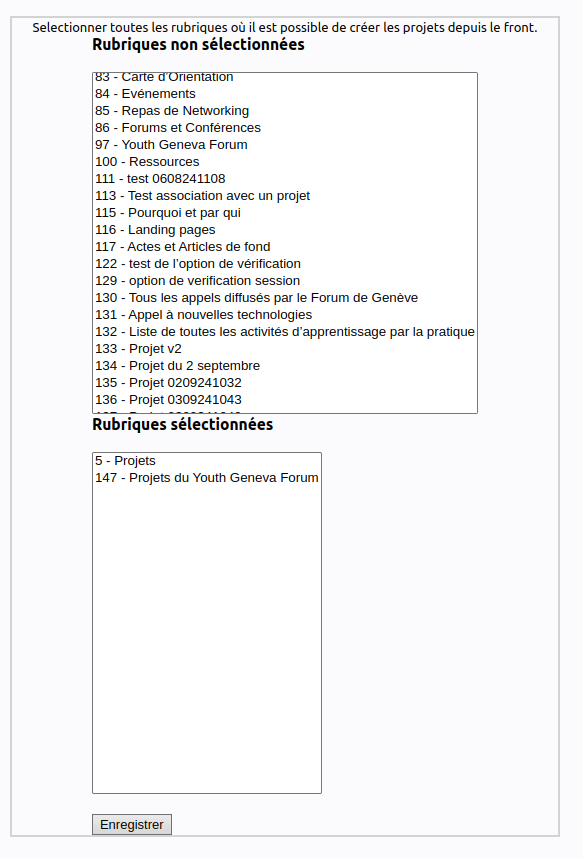
\includegraphics[trim=0 0 0 0, clip, width=0.4\textwidth]{./images/c1.png}
    \caption{Option 1 - Rubriques de création}
    \label{option1}
\end{figure}
\vspace{0.5cm}
% ///////////////////////////////////
\newpage

\textbf{Option 2 :} 
\begin{itemize}
    \item Configuration : \texttt{osip\_config\_demandes}
    \item Explication : Cette option limite la validation des demandes pour rejoindre un projet aux administrateurs du projet. Attention, il ne faut pas confondre un administrateur de projet et un administrateur SPIP.
\end{itemize}

\vspace{0.5cm}
\begin{figure}[h]
    \centering
    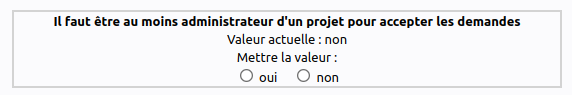
\includegraphics[trim=0 0 0 0, clip, width=1\textwidth]{./images/c2.png}
    \caption{Option 2 - Droits pour les demandes}
    \label{option2}
\end{figure}
\vspace{0.5cm}

% ///////////////////////////////////



\textbf{Option 3 :} 
\begin{itemize}
    \item Configuration : \texttt{osi\_projets/synchronisation\_mots}
    \item Explication : Dans le menu édition d'un projet, il existe la "\textit{Gestion des mots clés}" (Cf figure \ref{option3_bis}). Dans ce bloc, le premier bouton, intitulé "Mots-clés du projet", permet de synchroniser les mots-clés du projet à la rubrique associée (d'ajouter les mots clés du projet) et le deuxième l'inverse. Quand l'option 3 est activée, cette synchronisation prend en compte les groupes de mots-clés et ne rajoute que les mots-clés que l'autre groupe peut obtenir avec les règles des groupes de mots-clés.
\end{itemize}
\vspace{0.5cm}
\begin{figure}[h]
    \centering
    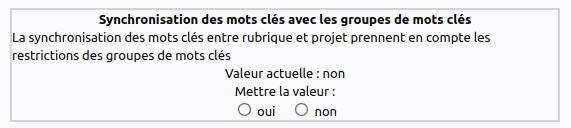
\includegraphics[trim=0 0 0 0, clip, width=1\textwidth]{./images/c3.png}
    \caption{Option 3 - Synchronisation avec les règles des groupes de mots}
    \label{option3}
\end{figure}
\vspace{0.5cm}
\begin{figure}[h]
    \centering
    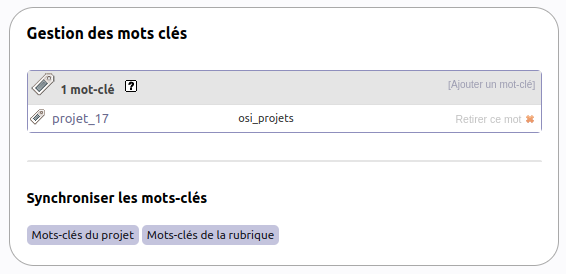
\includegraphics[trim=0 0 0 0, clip, width=0.7\textwidth]{./images/c3_bis.png}
    \caption{Menu de gestion des mots clés}
    \label{option3_bis}
\end{figure}

% ///////////////////////////////////
\newpage

\textbf{Option 4 :} 
\begin{itemize}
    \item Configuration : 
    \begin{itemize}
        \item \texttt{osi\_projets/types\_de\_mots/condition}
        \item \texttt{osi\_projets/types\_de\_mots/condition\_inverse}
        \item \texttt{osi\_projets/types\_de\_mots/recompense}
    \end{itemize}

    \item Explication : Dans le menu d'édition d'un projet, il est possible d'ajouter des mots clés à celui-ci. Dans la table \texttt{spip\_mots\_liens}, qui est la table qui permet de faire la liaison entre un mot et un objet (ici un projet), la colonne \texttt{lien\_projet} a été ajoutée. Cette colonne prend une valeur n qui permet de définir à quoi sert ce mot clé par rapport au projet.
    \begin{itemize}
        \item Conditions (n=2) : Les conditions sont des mots clés que l'auteur doit aussi avoir pour pouvoir rentrer dans le projet. Si l'auteur est déjà présent dans le projet mais qu'il ne respecte plus les conditions, rien n'est fait pour lui. Cependant, s'il y quitte le projet, il ne pourra plus revenir dedans tant qu'il ne respecte pas les nouvelles conditions. Ceci est possible grâce au filtre \texttt{filtre\_verifier\_conditions\_projet} utilisé dans le formulaire \texttt{ajouter\_auteur\_projet}, qui est le formulaire pour le front. Il faut donc faire attention, car le formulaire \texttt{ajouter\_autre\_auteur\_projet}, qui est celui utilisé dans le back office, permet lui en revanche d'ajouter un autre auteur dans le projet sans cette limitation.
        \item Conditions inverses (n=4) : Les conditions inverses fonctionnent avec le même principe que les conditions, sauf qu'ici il ne faut posséder aucune des conditions inverses pour rentrer dans un projet.
        \item Récompenses (n=3) : Les récompenses sont des mots clés que gagne un auteur quand, dans le menu édition du projet, on lui a donné les récompenses.
    \end{itemize}
\end{itemize}

\textbf{Remarque importante sur les récompenses :} Il faut faire attention avec les mots clés de "Récompenses". Dans l'état actuel du plugin, il est possible de "tricher" pour obtenir des mots clés de récompenses. En effet, un auteur peut ici créer un projet, ajouter autant de récompenses que de mots clés qu'il souhaite obtenir et se donner les récompenses (permission qu'il a car il est le créateur du projet). Dans l'état actuel du plugin, il est de la responsabilité du créateur du site de ne pas mettre en place un système de récompense s'il est possible de créer des projets sur le front par des personnes qui ne sont pas des personnes de confiance.


\vspace{0.5cm}
\begin{figure}[h]
    \centering
    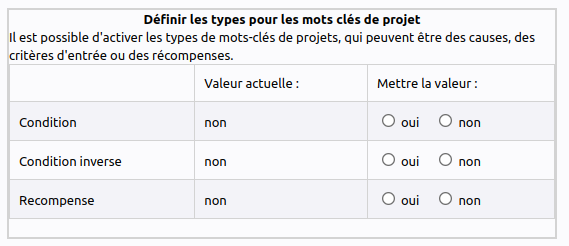
\includegraphics[trim=0 0 0 0, clip, width=1\textwidth]{./images/c4.png}
    \caption{Option 4 - Choix des types de mots clés}
    \label{option4}
\end{figure}
\vspace{0.5cm}


% ///////////////////////////////////


\textbf{Option 5 :} 
\begin{itemize}
    \item Configuration : \texttt{osi\_projets/verification\_projets}
    \item Explication : Cette option permet que tous les projets créés soient validés du côté back office pour les publier. Pour valider un projet, il faut se rendre dans la page d'édition des projets et modifier son statut.
\end{itemize}
\vspace{0.5cm}
\begin{figure}[h]
    \centering
    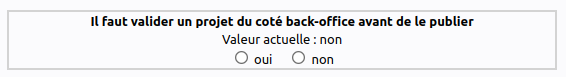
\includegraphics[trim=0 0 0 0, clip, width=1\textwidth]{./images/c5.png}
    \caption{Cadre de l'option 5}
    \label{option5}
\end{figure}
\vspace{0.5cm}

\newpage
% ///////////////////////////////////


\textbf{Option 6 :} 
\begin{itemize}
    \item Configuration : \texttt{osi\_projets/recursivite}
    \item Explication : Lors de la création d'un projet, un mot clé est ajouté à ce projet qui correspond à l'id du projet (c'est un mot clé unique qui représente ce projet). Si cette option est activée, alors pour tout nouveau sous-projet, le mot clé représentant le projet père est ajouté en tant que condition au projet fils. Le bouton "\textit{Appliquer la récurrence sur tous les projets déjà existants}" permet de faire cela aussi pour les anciens projets. Si on a plusieurs projets à la chaîne, les projets doivent se faire dans l'ordre du projet le plus haut au sous-projet le plus profond.
\end{itemize}
\vspace{0.5cm}
\begin{figure}[h]
    \centering
    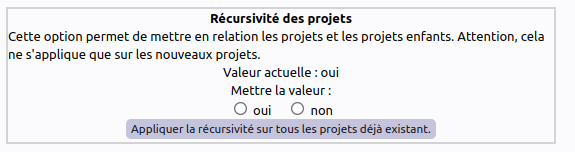
\includegraphics[trim=0 0 0 0, clip, width=1\textwidth]{./images/c6.png}
    \caption{Cadre de l'option 6}
    \label{option6}
\end{figure}
\vspace{0.5cm}

% ///////////////////////////////////

\textbf{Option 7 :} 
\begin{itemize}
    \item Configuration : \texttt{osi\_projets/webmaster\_droits}
    \item Explication : Cette option permet d'offrir les possibilités accordées aux administrateurs d'un projet aux administrateurs SPIP.
\end{itemize}
\vspace{0.5cm}
\begin{figure}[h]
    \centering
    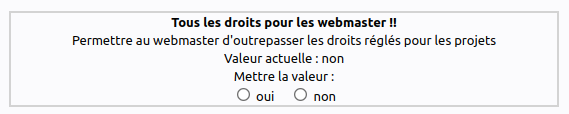
\includegraphics[trim=0 0 0 0, clip, width=1\textwidth]{./images/c7.png}
    \caption{Cadre de l'option 7}
    \label{option7}
\end{figure}

% ///////////////////////////////////
\newpage

\textbf{Option 8 :} 
\begin{itemize}
    \item Configuration : \texttt{osi\_projets/auteur\_banni}
    \item Explication : Cette option enlève tous les auteurs bannis de la liste des auteurs que l'on peut ajouter avec le formulaire \texttt{ajouter\_autre\_auteur\_projet}.
\end{itemize}
\vspace{0.5cm}
\begin{figure}[h]
    \centering
    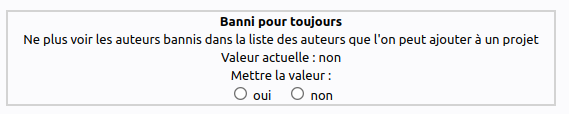
\includegraphics[trim=0 0 0 0, clip, width=1\textwidth]{./images/c8.png}
    \caption{Cadre de l'option 8}
    \label{option8}
\end{figure}

% ///////////////////////////////////

\textbf{Option 9 :} 
\begin{itemize}
    \item Configuration : \texttt{osi\_projets/creer\_sous\_projet\_int}
    \item Explication : Cette option permet aux administrateurs d'un projet de pouvoir créer un sous-projet sur le front. Cette utilisation est supplémentaire à celle de l'option 1.
\end{itemize}
\vspace{0.5cm}
\begin{figure}[h]
    \centering
    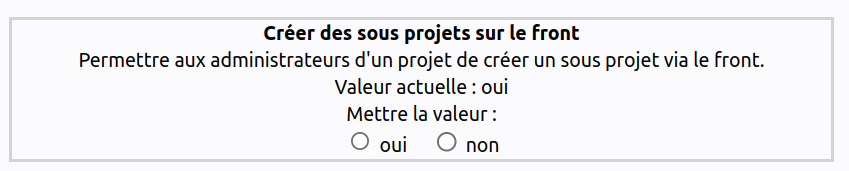
\includegraphics[trim=0 0 0 0, clip, width=1\textwidth]{./images/c9.png}
    \caption{Cadre de l'option 9}
    \label{option9}
\end{figure}


% ///////////////////////////////////
\newpage

\textbf{Option 10 :} 
\begin{itemize}
    \item Explication : Cette option est une sécurité qui permet de situer le projet sur le front quand aucune rubrique mère n'est définie lors de la création du projet. Si aucune rubrique n'est définie ici, le projet sera créé dans le sommaire.
\end{itemize}
\vspace{0.5cm}
\begin{figure}[h]
    \centering
    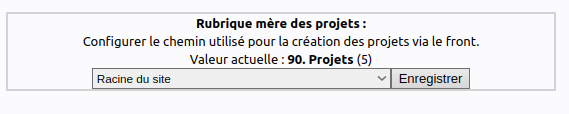
\includegraphics[trim=0 0 0 0, clip, width=1\textwidth]{./images/c10.png}
    \caption{Cadre de l'option 10}
    \label{option10}
\end{figure}

% ///////////////////////////////////
\newpage

\subsubsection*{Gestion des rôles} \label{subsubsection:gestion-roles}

Chaque membre d'un projet peut obtenir des rôles. Les rôles sont liés à un membre d'un projet. C'est-à-dire qu'un auteur peut avoir un rôle pour un projet et ne pas l'avoir pour un autre projet.\\
\newline
Le fichier \texttt{action/exemple\_roles} permet de voir la forme que peuvent avoir des rôles. Il est activable sur le back-office grâce au bouton "\textit{Utiliser les rôles d'exemple}". Les rôles d'exemple sont les suivants :


\vspace{0.5cm}

\begin{tabular}{|>{\centering\arraybackslash}m{6.2cm}|>{\centering\arraybackslash}m{6cm}|}
    \hline
    \rowcolor{lightgray} 
    Nom du rôle & Utilisation \\ 
    \hline
    \textbf{FORMATEUR} & Représente les personnes qui réalisent les formations \\ 
    \hline
    \textbf{SPONSOR} & Représente les personnes qui financent les projets \\ 
    \hline
    \textbf{EVALUATEUR PAR LES PAIRS} & Personne en lien avec le projet et qui sert à l'évaluer \\ 
    \hline
    \textbf{EVALUATEUR INDEPENDANT} & Personne pas directement en lien avec le projet et qui sert à l'évaluer \\ 
    \hline
\end{tabular}

\vspace{0.5cm}

Cependant, le but n'est pas forcément d'utiliser les rôles d'exemple, mais plutôt de créer des rôles adaptées à l'utilisation du plugin.\\
\newline
Un rôle possède trois caractéristiques.
\begin{itemize}
    \item Le titre du rôle (obligatoire) : cela permet de l'identifier, on ne peut pas avoir deux rôles avec le même titre.
    \item La description du rôle : permet d'expliquer le but du rôle.
    \item La question : c'est la question qui est posée dans le formulaire de demande pour rejoindre le projet (\textit{ajouter\_auteur\_projet}) pour rejoindre avec ce rôle. 
\end{itemize}
Une fois qu'un rôle est créé, il faut penser à cliquer sur le bouton "\textit{Rendre le rôle actif}" pour pouvoir utiliser le rôle. Initialement, le rôle est inactif.

\subsubsection*{Gestion des notifications} \label{subsubsection:gestion-notifications}

Pour pouvoir utiliser la partie notification du plugin, il faut installer le plugin \href{https://plugins.spip.net/notifavancees.html}{Notifications avancées}.\\
\newline
Il existe deux types de notifications : les notifications individuelles et les notifications de groupe. Les notifications individuelles s'adressent à la personne qui est concernée, généralement la personne qui essaie de rejoindre un projet. Les notifications de groupe s'adressent ici à l'ensemble des personnes du projet.\\
\newline
Les notifications se trouvent toutes dans la rubrique \textit{notifications}.

\subsection{Menu édition} \label{subsection:menu-edition}

Dans le menu d'édition, on retrouve les différentes possibilités de gestion et de modification d'un projet précis.

\begin{itemize}
    \item La gestion des mots clés : permet de rajouter un mot clé et de modifier son type (Cf. option 4).
    \item La gestion des demandes : on trouve ici les demandes pour rejoindre le projet et les demandes pour obtenir un rôle. Seuls les membres ayant au minimum des droits administrateurs peuvent accepter (ou refuser) les demandes. 
    \item La gestion des membres du projet : permet de modifier le rôle ou les droits d'un membre d'un projet. C'est aussi ici qu'on peut exclure un membre du projet.
\end{itemize}


\newpage

\section{Fonctionnement du plugin} \label{section:fonctionnement}
\subsection{Droits sur un projet}

Par rapport à un projet, nous avons différents participants. On peut regrouper ces participants en 3 niveaux.
\begin{itemize}
    \item \textbf{Le créateur du projet}, ou super-administrateur, est l'utilisateur qui a décidé de créer le projet. Il possède tous les droits sur ce projet et est le seul capable de supprimer le projet.
    \item \textbf{Les administrateurs} sont des utilisateurs qui possèdent différents droits sur ce projet. Ils peuvent accepter ou refuser les demandes pour rejoindre le projet. Ils peuvent agir sur les caractéristiques d'un membre standard du projet. Ils n'ont pas les droits pour agir directement sur les autres administrateurs du projet.
    \item \textbf{Membre standard} regroupe les utilisateurs qui participent au projet et qui n'ont pas de droit particulier.
\end{itemize}

\framebox{
    \begin{minipage}{\dimexpr\textwidth-2\fboxsep-2\fboxrule\relax}
        \textbf{Remarque :}\\
        Les niveaux de droits sur un projet sont indépendants des niveaux de droits d'un auteur SPIP. Les administrateurs du site SPIP ont des droits de \textit{super-administrateur} sur les projets avec l'option 7. Les rédacteurs et visiteurs ont des droits standards, c'est-à-dire ceux définis directement dans le projet. 
    \end{minipage}
}

\subsection{Conditions et récompenses}

Une des possibilités d'utilisation de ce plugin est de voir les projets comme des formations. En voyant cela ainsi, il peut être logique d'imaginer des conditions d'entrée et des récompenses par rapport à la participation à un projet. Cette utilisation est possible via un système de mots-clés présenté dans l'option 4.

\subsection{Récursivité}

Une des possibilités est de permettre la participation à des projets, mais dans un ordre précis. Cette manière de voir les choses se rapproche de l'utilisation de l'option 6 (un utilisateur ne peut pas rejoindre un projet tant qu'il n'a pas validé le projet racine).\\
\newline
Dans le cas où un projet demande déjà des critères d'entrée, la récurrence des projets est une condition supplémentaire à valider pour participer au projet.


\newpage

\section{Contenu du plugin} \label{section:contenu}

\subsection{Balises}

On rappelle que l'on peut appeler une balise avec la notation \texttt{\#NOM\_DE\_LA\_BALISE}. Voici la liste des balises du plugin dans sa version actuelle :

\vspace{0.5cm}

% \begin{tabular}{|C{6.2cm}|C{3cm}|C{6cm}|}
\begin{tabular}{|>{\centering\arraybackslash}m{6.2cm}|>{\centering\arraybackslash}m{3cm}|>{\centering\arraybackslash}m{6cm}|}
    \hline
    \rowcolor{lightgray} 
    Nom de la balise & Arguments & Description \\ 
    \hline
    \textbf{OSIP\_AUTEUR\_DU\_PROJET} & id\_projet & Permet de récupérer le créateur du projet \\ 
    \hline
    \textbf{OSIP\_DEBUG\_NB\_PROJETS} & / & Permet de récupérer le nombre de projets dans la base de données \\ 
    \hline
    \textbf{OSIP\_DEBUG\_NB\_RUBRIQUES} & / & Permet de récupérer le nombre de rubriques associés à des projets dans la base de données \\ 
    \hline
    \textbf{OSIP\_ETAT\_LIEN\_PROJET} & / & Permet de récupérer l'état d'un membre (ses droits) \\ 
    \hline
    \textbf{OSIP\_LISTE\_ADMINISTRATEURS} & id\_projet & Permet de récupérer l'ensemble des administrateurs d'un projet.\\
    \hline
    \textbf{OSIP\_LISTE\_AUTEURS} & id\_projet & Permet de récupérer l'ensemble des auteurs associés à un projet \\

    \hline
    \textbf{OSIP\_LISTE\_AUTEURS\_VALEUR} & id\_projet, valeur & Permet de récupérer l'ensemble des auteurs avec des droits de correspondant à la valeur \\
    \hline
    \textbf{OSIP\_LISTE\_MEMBRES} & id\_projet & Permet de récupérer l'ensemble des auteurs avec des droits de membres d'un projet \\
    \hline
    \textbf{OSIP\_LISTE\_PROJETS} & id\_auteur & Permet de récupérer l'ensemble des projets d'un auteur \\ 
    \hline
    \textbf{OSIP\_MOTS} & id\_projet & Permet de récupérer l'ensemble des mots clés d'un projet \\
    \hline
    \textbf{OSIP\_NB\_AUTEURS} & id\_projet & Permet de récupérer le nombre d'auteur dans le projet \\
    \hline
    \textbf{OSIP\_NB\_DEMANDES} & id\_projet & Permet de récupérer le nombre de demandes dans un projet \\
    \hline
    \textbf{OSIP\_NB\_PROJETS} & / & Permet de récupérer le nombre de projets actifs \\ 
    \hline
\end{tabular}

\newpage

\subsection{Filtres}

Les filtres sont nécessaires pour personnaliser dynamiquement les squelettes du site. En effet, on peut imaginer utiliser un filtre de la manière suivante. 

\vspace{0.2cm}

\begin{lstlisting}

    [(#SESSION\{id_auteur\}|filtre_verifier_auteur_projet\{#ID_PROJET\}|oui)
        L'auteur appartient au projet
    ]
    [(#SESSION\{id_auteur\}|filtre_verifier_auteur_projet\{#ID_PROJET\}|non)
        L'auteur n'appartient pas au projet
    ]

\end{lstlisting}

\vspace{0.4cm}

\framebox{
    \begin{minipage}{\dimexpr\textwidth-2\fboxsep-2\fboxrule\relax}
        \textbf{Remarque:}\\
        Spip ne supporte pas forcément l'utilisation de filtres lorsqu'il y a une boucle à l'intérieur. Pour résoudre cela, il faut fermer le filtre avant le début de la boucle, l'ouvrir dans la boucle et le fermer avant la fin, puis le ré-ouvrir après la boucle. 
    \end{minipage}
}

\vspace{0.5cm}

Dans ce plugin, deux familles de filtres ont été utilisées :
\begin{itemize}
    \item Des filtres GETTER pour récupérer certaines informations des tables
    \item Des filtres de VÉRIFICATION pour rendre le code dynamique comme dans l'exemple précédent.
\end{itemize}
Nous allons voir les filtres les plus importants pour le front, qui sont les filtres de VÉRIFICATION. En voici une liste non exhaustive.

\vspace{0.5cm}

\begin{tabular}{|>{\centering\arraybackslash}m{6.2cm}|>{\centering\arraybackslash}m{3cm}|>{\centering\arraybackslash}m{6cm}|}
    \hline
    \rowcolor{lightgray} 
    Nom du filtre & Arguments & Description \\ 
    \hline
    \textbf{filtre\_verifier\_createur\_projet} & id\_auteur \newline id\_projet & Permet de vérifier qu'un auteur est le createur du projet. \\ 
    \hline
    \textbf{filtre\_verifier\_administrateur\_projet} & id\_auteur \newline id\_projet & Permet de vérifier qu'un auteur est administrateur du projet. \\ 
    \hline
    \textbf{filtre\_verifier\_membre\_projet} & id\_auteur \newline id\_projet & Permet de vérifier qu'un auteur est membre du projet. \\ 
    \hline
    \textbf{filtre\_verifier\_auteur\_projet} & id\_auteur \newline id\_projet & Permet de vérifier qu'un auteur appartient au projet (membre, administrateur, createur). \\ 
    \hline
    \textbf{filtre\_verifier\_droits\_projet} & id\_auteur \newline id\_projet & Filtre qui permet de vérifier qu’un auteur a au moins les droits d'administrateur. \\ 
    \hline
    \textbf{filtre\_verifier\_droits\_demandes \newline \_configuration} & id\_auteur \newline id\_projet & Filtre qui permet de vérifier les droits nécessaires pour accepter les demandes. \\ 
    \hline
    \textbf{filtre\_verifier\_demande} & id\_auteur \newline id\_projet & Permet de vérifier qu'un auteur à fait une demande pour rejoindre un projet \\ 
    \hline
    \textbf{filtre\_verifier\_demande\_echec} & id\_auteur \newline id\_projet & Permet de vérifier qu'un auteur à fait une demande qui a été refusé. \\ 
    \hline
    \textbf{filtre\_verifier\_auteur\_banni} & id\_auteur \newline id\_projet & Permet de vérifier qu'un auteur a été banni du projet. \\ 
    \hline
    \textbf{filtre\_verifier\_rubrique\_projet} & id\_rubrique & Permet de vérifier que la rubrique est bien une rubrique d'un projet \\ 
    \hline
    \textbf{filtre\_verifier\_conditions\_projet} & id\_auteur \newline id\_projet & Filtre pour vérifier que les conditions d'un projet sont respectées par l'auteur. \\ 
    \hline
    \textbf{filtre\_verifier\_conditions\_role} & id\_auteur \newline id\_role & Filtre pour vérifier que les conditions d'un role sont respectées par l'auteur. \\ 
    \hline
\end{tabular}

\vspace{0.5cm}

\newpage

\subsection{Formulaires}

On rappelle que l'on peut appeler un formulaire avec la notation \texttt{\#FORMULAIRE\_NOM\_DU\_FORMULAIRE}. Les arguments du tableau suivant ne représentent pas les caractéristiques du formulaire mais juste les arguments donnés en plus. Voici une liste non exhaustive des formulaires du plugin dans sa version actuelle, on ne citera pas ici les formulaires de configuration. 
\vspace{0.5cm}
\begin{tabular}{|>{\centering\arraybackslash}m{6.2cm}|>{\centering\arraybackslash}m{3cm}|>{\centering\arraybackslash}m{6cm}|}
    \hline
    \rowcolor{lightgray} 
    Nom du formulaire & Arguments & Description \\ 
    \hline
    \textbf{AJOUTER\_AUTEUR\_PROJET} & id\_projet\newline id\_auteur & Permet de rajouter un auteur à un projet. On prend en compte ici des conditions. \\ 
    \hline
    \textbf{AJOUTER\_AUTRE\_AUTEUR\_PROJET} & id\_projet & Permet de rajouter un auteur precis à un projet. On ne prend pas en compte ici des conditions \\ 
    \hline
    \textbf{CHANGER\_CHAMP\_PROJET} & 
    id\_auteur\_projet
    \newline
    champ
    \newline
    valeur
    \newline
    texte\_bouton
    & Permet modifier un champ d'un membre d'un projet (définie grace à id\_auteur\_projet) afin de mettre une certaine valeur.\\ 
    \hline
    \textbf{CHANGER\_VALEUR\_ROLE} & 
    id\_role
    \newline
    id\_auteur\_projet
    \newline
    valeur
    \newline
    texte\_bouton
    & Permet d'accorder ou non un rôle à un participant à un projet.\\ 
    \hline
    \textbf{CLASSER\_MOT} & 
    id\_mot
    \newline
    id\_objet
    \newline
    nom\_objet
    \newline
    texte\_bouton
    & Permet de modifier le type d'un mot par rapport à un objet (Cf option 4)\\ 
    \hline
    \textbf{CREER\_UN\_PROJET} & id\_auteur & Permet de créer un projet. L'auteur qui créer le projet devient "createur" sur ce projet.\\
    \hline
    \textbf{CREER\_UN\_ROLE} & / & Permet de créer un nouveau rôle\\
    \hline
    \textbf{DEMANDER\_UN\_ROLE} & 
    id\_projet
    \newline
    id\_auteurs
    \newline
    id\_role
     & Permet à un auteur de demander un nouveau rôle\\
    \hline
    \textbf{DONNER\_RECOMPENSES} & 
    id\_projet
    & Permet de donner l'ensemble des récompenses d'un projet à un auteur. Cela lui accorde les mots clés.\\
    \hline
    \textbf{MODIFIER\_POSITION\_DU\_PROJET} & 
    id\_projet
    & Permet de modifier l'emplacement d'un projet. Ceci est à éviter surtout dans le cas d'une utilisation front du plugin.\\
    \hline
    \textbf{PERSONNALISER\_PROJET} & 
    id\_projet
    & Modifie l'ensemble des caractéristiques front d'un projet.\\
    \hline
\end{tabular}

\newpage

\vspace{0.5cm}

\framebox{
    \begin{minipage}{\dimexpr\textwidth-2\fboxsep-2\fboxrule\relax}
        \textbf{Remarque :}\\
        Le formulaire \textbf{CHANGER\_CHAMP\_PROJET} est un formulaire très puissant car c'est lui qui permet de modifier n'importe quelle information d'un participant à un projet (information de la table \texttt{spip\_auteur\_projet}). Il ne peut donc pas être utilisé en demandant à l'utilisateur de rentrer le champ et la valeur par mesure de sécurité au risque de se voir supprimer le membre. Il faut utiliser ce formulaire comme un bouton.\\
        \newline
        Voici un exemple d'utilisation :
        \begin{center}
            \texttt{\#FORMULAIRE\_CHANGER\_CHAMP\_PROJET\{\#ID\_AUTEUR\_PROJET, etat, 1, affichage\_etat\}}
        \end{center}
    \end{minipage}
}



\newpage

\section{Structure du plugin} \label{section:structure}
Etant donné que ce plugin doit pouvoir s'intégrer aux différents sites SPIP, il doit pouvoir utiliser les systèmes déjà mis en place. Les nouvelles tables ajoutées pour le fonctionnement de ce plugin se rattachent donc à des tables déjà existantes du système SPIP.\\
\newline
On retrouve les différentes tables suivantes :

\vspace{0.5cm}

\begin{figure}[h]
    \centering
    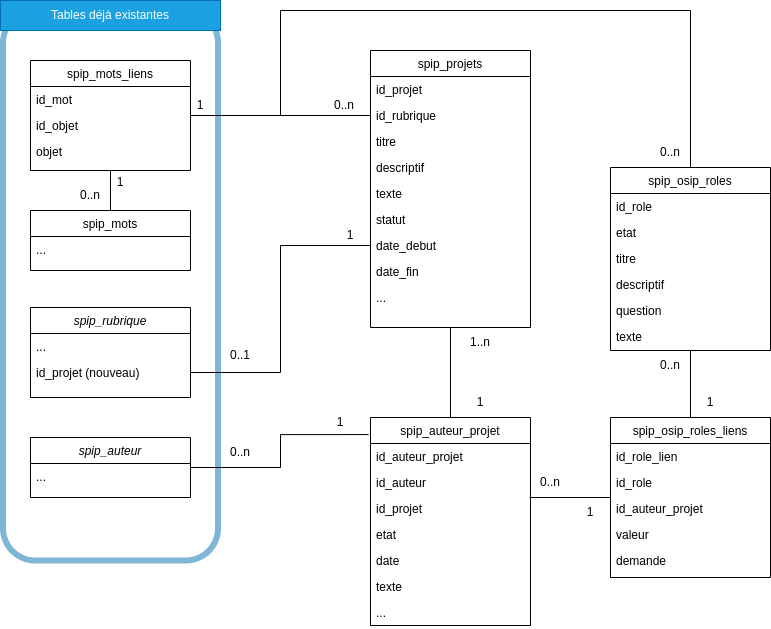
\includegraphics[trim=0 0 0 0, clip, width=1\textwidth]{images/table_plugin_projet.drawio.png}
    \caption{Tables du plugins "OSI\_Projets"}
    \label{Tables du plugin osiprojets}
\end{figure}
\newpage
On peut voir que ce plugin fonctionne grâce à quatre nouvelles tables : 
\begin{itemize}
    \item \texttt{spip\_projets} : Table qui représente les "projets" (groupe d'auteurs). L'idée est ici de se rattacher à un type de page déjà présent sur le front (ici une rubrique) pour pouvoir profiter des fonctionnalités déjà présentes sur cette dernière en ajoutant celles nécessaires pour le fonctionnement du plugin.
    \item \texttt{spip\_auteur\_projet} : Table qui représente le lien entre un auteur et un projet. L'état permet de représenter les différents niveaux de droits sur le projet. Cette table représente aussi les demandes pour rejoindre un projet.
    \item \texttt{spip\_osip\_roles} : Table qui représente des rôles que peuvent obtenir les membres d'un projet.
    \item \texttt{spip\_osip\_roles\_liens} : Table qui représente le lien entre un rôle et un membre d'un projet. C'est aussi la table qui représente les demandes pour obtenir un rôle ou non. 
\end{itemize}
En regardant les tables de la figure \ref{Tables du plugin osiprojets}, on peut voir qu'un projet peut accueillir autant d'auteurs que possible, mais avec un minimum d'un auteur (le créateur du projet). \\
\newline
Comme il a été dit précédemment, le niveau de droit d'un utilisateur par rapport à un projet est réalisé grâce à la colonne \texttt{etat} d'un élément de la table \textit{spip\_auteur\_projet}. En effet, on retrouve les niveaux d'état suivants : 
\begin{itemize}
    \item 3 - Créateur du projet
    \item 2 - Administrateur du projet
    \item 1 - Membre du projet
    \item 0 - Utilisateur ayant fait une demande pour rejoindre le projet
    \item -1 - Utilisateur ayant fait une demande pour rejoindre le projet qui a été refusée
    \item -2 - Utilisateur qui a été banni du projet
\end{itemize}






\newpage
% \newpage
% \section{Annexes} \label{section:annexes}
\newpage
% \newpage
% \begin{thebibliography}{1}
%     \bibitem{exemple}
%     exemple - \href{https://exemple.fr}{https://exemple.fr}
% \end{thebibliography}


% ///////////////////////////////////////////////////

\end{document}